%9T5
\begin{dang}{Số lượng và vị trí của cực đại – cực tiểu}
\Anlythuyet{
\circEX{1} Số cực đại, cực tiểu trên đoạn giữa hai nguồn $S_1S_2=\ell$
\begin{itemize}
\item Số cực đại thỏa mãn: 
$\boder{-\dfrac{\ell}{\lambda}< k< \dfrac{\ell}{\lambda}}\quad (k\in\mathbb{Z})$
\item Số cực tiểu thỏa mãn: $\boder{-\dfrac{\ell}{\lambda}-\dfrac{1}{2}<  k< \dfrac{\ell}{\lambda}-\dfrac{1}{2}}\quad (k\in\mathbb{Z})$
\end{itemize}
\circEX{2} Số cực đại, cực tiểu trên đoạn thẳng MN bất kì
\immini{\begin{itemize}
\item Xét hai điểm M, N về cùng một phía và cách hai nguồn sóng kết hợp \bth{A, B} cho trước các khoảng \bth{d_{1M},\ d_{2M},\ d_{1N},\ d_{2N}}. 
\item Đặt $\Delta d_M = d_{1M}-d_{2M}$ và $\Delta d_N = d_{1N}-d_{2N}$. Giả sử $\Delta d_M<\Delta d_N$. 
\item Một điểm trong vùng giao thoa thuộc MN khi  $\Delta d_M \le d_1 - d_2\le \Delta d_N$
\begin{itemize}
\item Số điểm (đường) cực đại:  $\boder{\dfrac{\Delta d_M}{\lambda}\le k\le \dfrac{\Delta d_N}{\lambda}}\quad (k\in\mathbb{Z})$.
\item Số điểm (đường) cực tiểu: $\boder{\dfrac{\Delta d_M}{\lambda}-\dfrac{1}{2}\le k\le \dfrac{\Delta d_N}{\lambda}-\dfrac{1}{2}}\quad (k\in\mathbb{Z})$
\end{itemize}
\end{itemize}}{\begin{tikzpicture}
\tkzDefPoints{0/0/a, 4/0/b, 1/2/n, 2.2/2.5/m}
\tkzDrawSegments[dashed](a,b a,m b,m a,n b,n)
\tkzDrawPoints[size=3,fill=white](a,b,m,n)
\tkzLabelSegment[above left](a,n){$d_{1M}$}
\tkzLabelSegment[below](b,n){$d_{2M}$}
\tkzLabelSegment[below=5pt](a,m){$d_{1N}$}
\tkzLabelSegment[above right](b,m){$d_{2N}$}
\tkzLabelPoint[below](a){$A$}
\tkzLabelPoint[below](b){$B$}
\tkzLabelPoint[above](m){$N$}
\tkzLabelPoint[above](n){$M$}
\end{tikzpicture}}
\Note{
\begin{itemize}
\item \textit{Trong các công thức trên nếu không xét tại M và tại N hoặc M và N trùng với nguồn thì bỏ đi dấu "="}
\item \textit{Công thức trên sẽ sai khi MN cắt đường hypebol tại hai điểm, trường hợp này rất ít khi xảy ra}
\end{itemize}
}
\circEX{2}  Số cực đại, cực tiểu trên đường tròn, elip hoặc hình vuông
\immini{\begin{itemize}
\item Tìm số đường cực đại (hoặc cực tiểu) trên đoạn thẳng MN thuộc đoạn hai nguồn và nằm trong đường tròn, elip hoặc hình vuông đó. 
\item Số giao điểm của các đường cực đại (hoặc cực tiểu) với đường tròn, elip hoặc hình vuông chính là số điểm cần tìm.
\end{itemize}}{\begin{tikzpicture}[scale=1]
\begin{scope}[shift={(0,0)}]
\tkzInit[ymin=-2,ymax=2,xmin=-3,xmax=3]\tkzClip
\tkzDefPoints{-2/0/s1, 2/0/s2, -0.4/0/m, 1.4/0/n}
\draw[red] plot[domain=-2:2] ({1*cosh(\x)-0.75},{5*sinh(\x)});
\draw[red] plot[domain=-2:2] ({-1*cosh(\x)+0.75},{5*sinh(\x)});
\draw[red] plot[domain=-2:2] ({1*cosh(\x)-0.5},{3*sinh(\x)});
\draw[red] plot[domain=-2:2] ({-1*cosh(\x)+0.5},{3*sinh(\x)});
\draw[red] plot[domain=-2:2] ({1*cosh(\x)-0.25},{2.2*sinh(\x)});
\draw[red] plot[domain=-2:2] ({-1*cosh(\x)+0.25},{2.2*sinh(\x)});
\draw[red] plot[domain=-2:2] ({1*cosh(\x)+0.25},{1.3*sinh(\x)});
\draw[red] plot[domain=-2:2] ({-1*cosh(\x)-0.25},{1.3*sinh(\x)});
\draw[red] plot[domain=-2:2] ({1*cosh(\x)},{1.75*sinh(\x)});
\draw[red] plot[domain=-2:2] ({-1*cosh(\x)},{1.75*sinh(\x)});
\draw[red] plot[domain=-2:2] ({1*cosh(\x)+0.5},{1.01*sinh(\x)});
\draw[red] plot[domain=-2:2] ({-1*cosh(\x)-0.5},{1.01*sinh(\x)});
\draw[red](0,3)--(0,-3);
\draw[blue](s1)--(s2);
\tkzLabelPoint[left](s1){$A$}
\tkzLabelPoint[right](s2){$B$}
\tkzDrawCircle[diameter,color=blue](m,n)
\tkzDrawPoints[size=3,fill=white](m,n,s1,s2)
\tkzLabelPoint[above left](m){$M$}
\tkzLabelPoint[above right](n){$N$}
\end{scope}
\end{tikzpicture}}
}
\end{dang}
